\documentclass[12pt, a4paper, oneside, fontset=windows]{ctexbook}
\usepackage{amsmath, amsthm, amssymb, bm, graphicx, hyperref, mathrsfs}
% 让图像路径兼容从仓库根目录编译
\graphicspath{{./一维随机游动/}{./}}
\usepackage{tcolorbox}
\usepackage{tikz}
\usetikzlibrary{tikzmark, arrows.meta, shapes}
\usepackage{geometry}
\geometry{a4paper, margin=1in}
\setlength{\parindent}{0pt}
\setlength{\parskip}{1em}

\title{{\Huge{一维随机游动}}\\课程笔记附录:解题过程图示}
\author{刘明琦}
\date{\today}
\linespread{1.3}

% 定理环境(与仓库统一)
\newtheorem{theorem}{定理}[section]
\newtheorem{definition}{定义}[section]
\newtheorem{lemma}[theorem]{引理}
\newtheorem{corollary}[theorem]{推论}
\newtheorem{example}{例}[section]
\newtheorem{proposition}[theorem]{命题}

% 常用算子(与仓库统一)
\DeclareMathOperator*{\esssup}{ess\,sup}
\DeclareMathOperator{\st}{\mathrm{s.t.}}
\DeclareMathOperator{\diff}{\mathrm{i.f.f.}}
\DeclareMathOperator{\ie}{\mathrm{i.e.}}

\begin{document}

\maketitle

\pagenumbering{roman}
\setcounter{page}{1}
\begin{center}
	\Huge\textbf{前言}
\end{center}~\\
本附件整理了“一维随机游动”问题的解题过程要点,并配套展示了五张过程图示(1.jpg–5.jpg)。为保持与主笔记一致,采用 XeLaTeX 与统一的版式和环境设置。

\begin{flushright}
	\begin{tabular}{c}
		刘明琦\\
			oday
	\end{tabular}
\end{flushright}

\newpage
\pagenumbering{Roman}
\setcounter{page}{1}
	ableofcontents
\newpage
\setcounter{page}{1}
\pagenumbering{arabic}

\chapter{问题与解答概览}

\begin{tcolorbox}
	extbf{问题背景(概述)}\\
考虑一维随机游动:粒子以步长 $\pm 1$(或一般步长)在整数线上移动。典型关注量包括:首次到达某点的概率、预期返回时间、吸收边界下的吸收概率与期望步数、偏置游动的极限行为等。本章仅整理图示步骤,不替代完整推导。
\end{tcolorbox}

\section{解题过程图示}
下列图示按解题顺序排列。若需插入文字注释或推导公式,可在对应图之后添加段落或公式环境。

\begin{figure}[h]
	\centering
	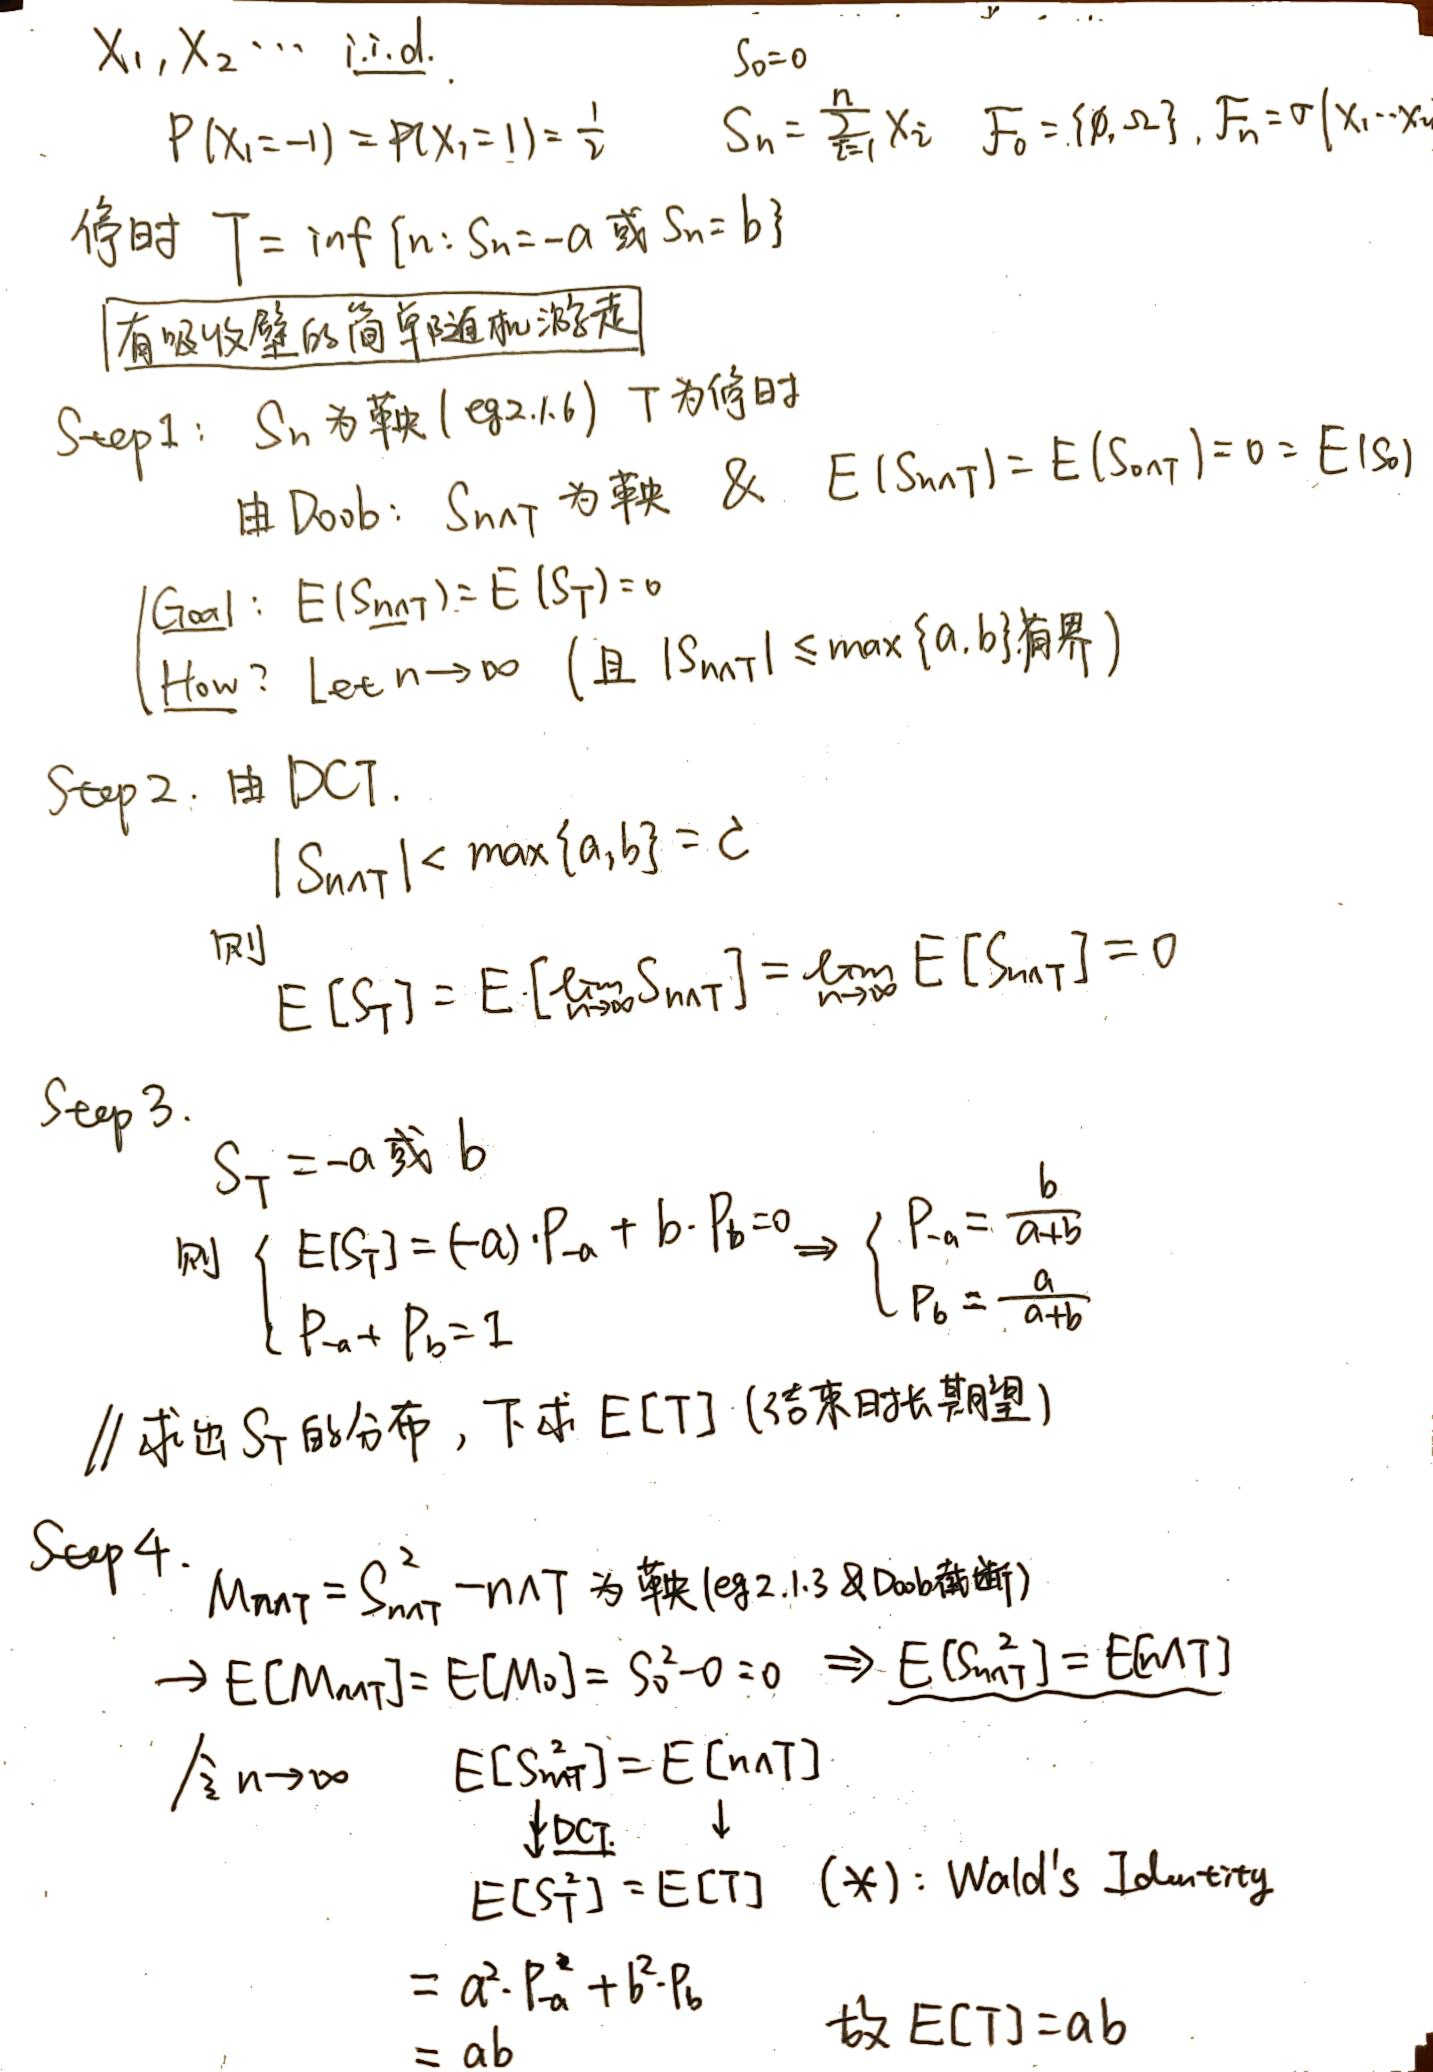
\includegraphics[width=0.92\textwidth]{1.jpg}
	\caption{步骤 1:问题建模与基本设定(示意)}\label{fig:rw-step1}
\end{figure}

\begin{figure}[h]
	\centering
	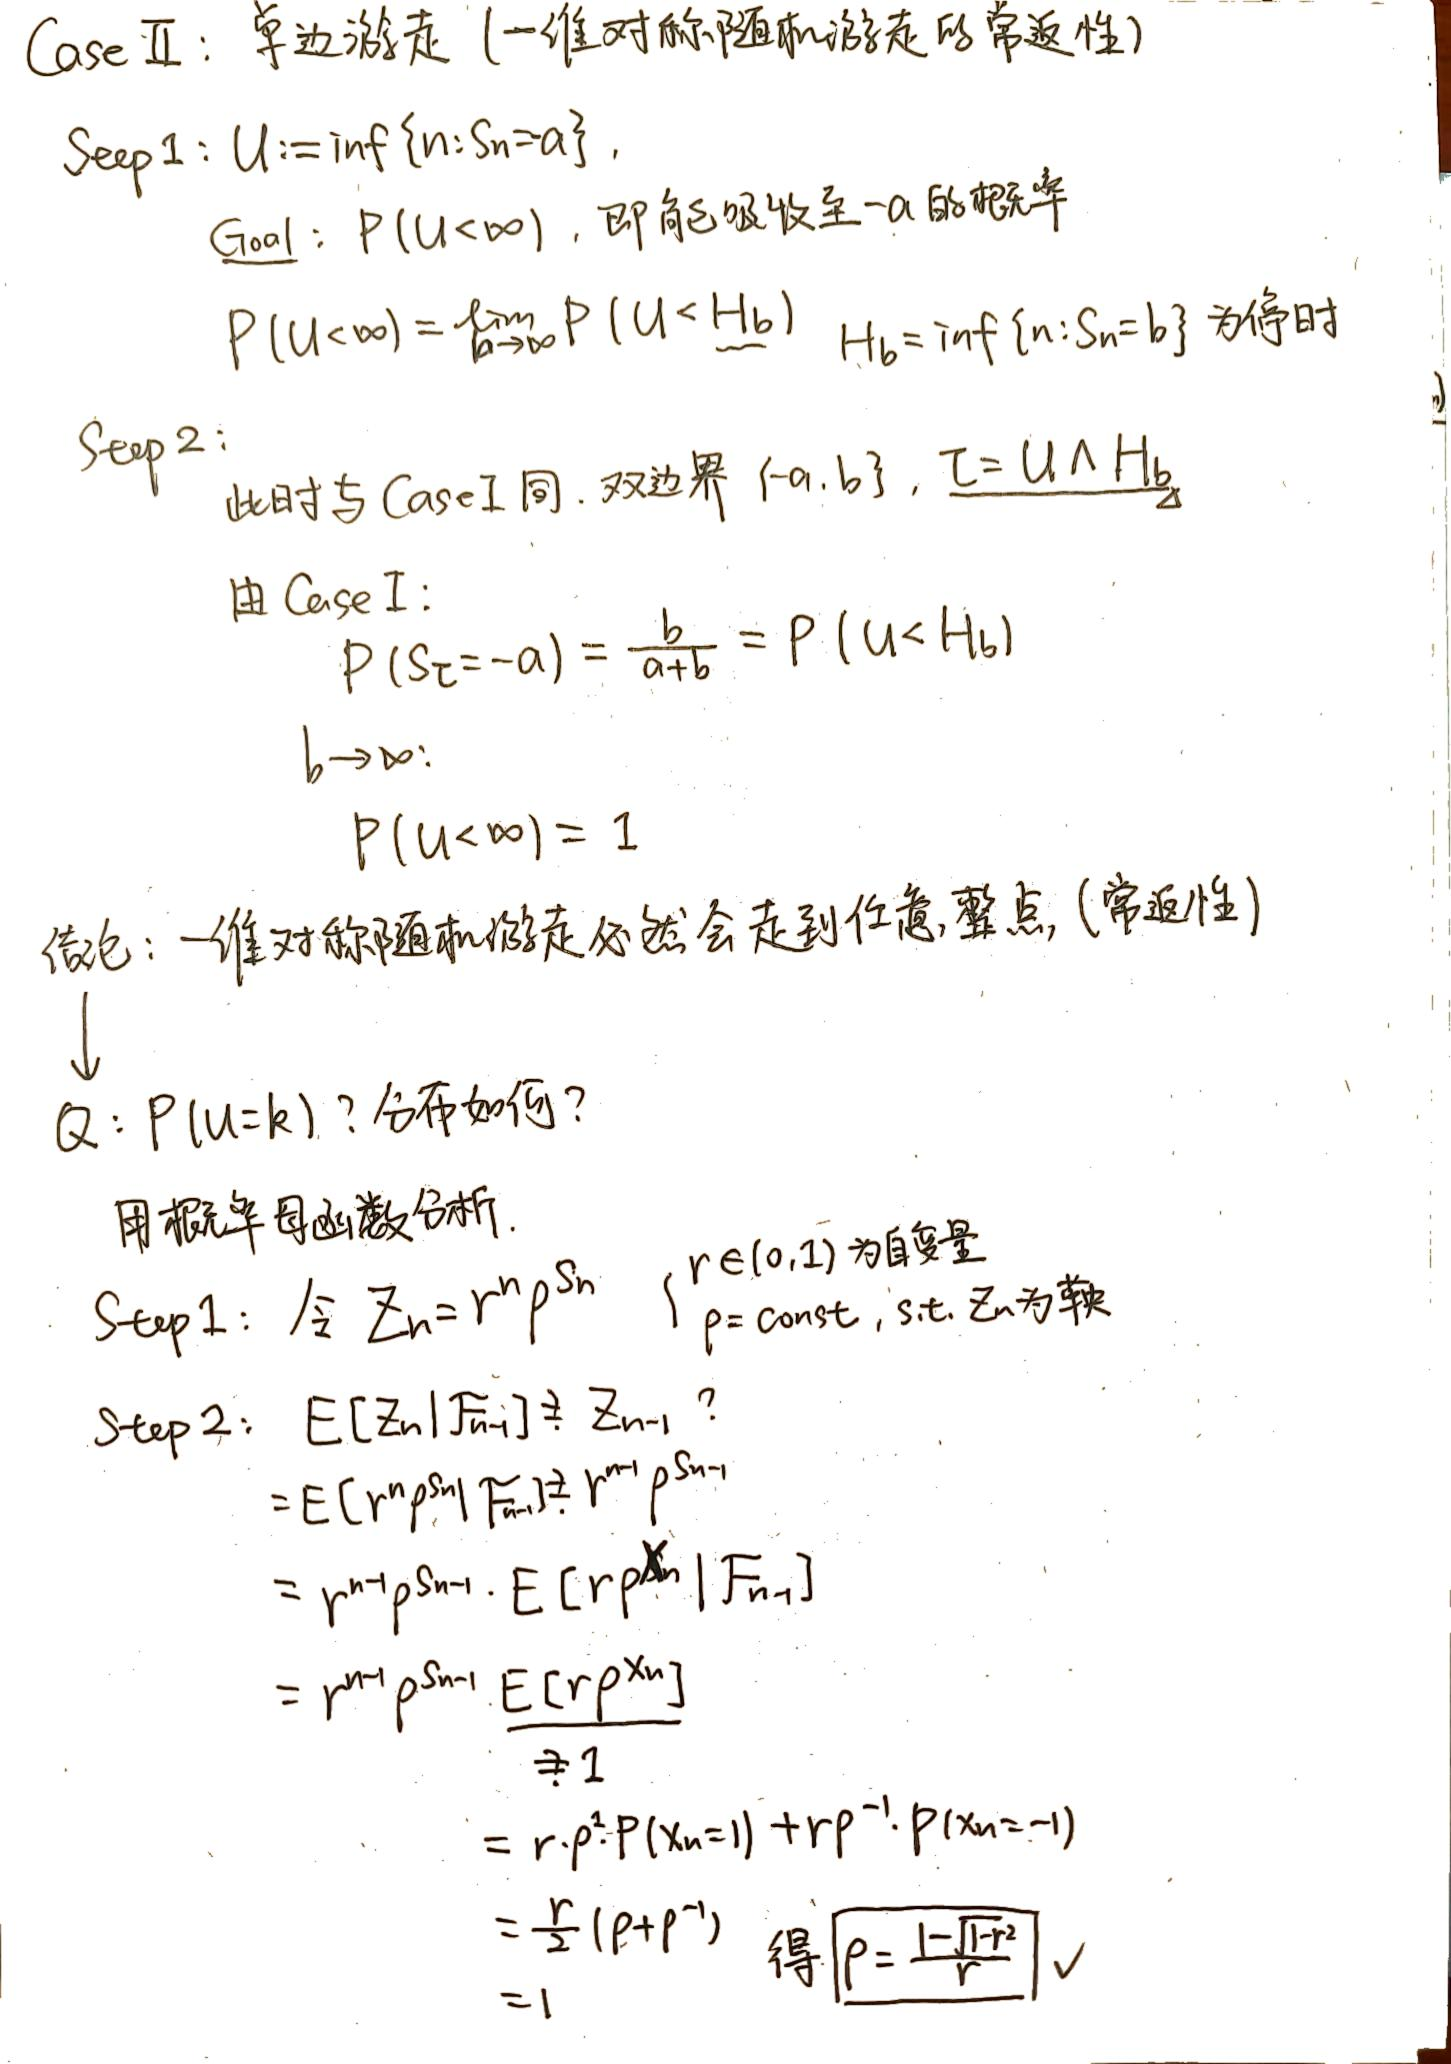
\includegraphics[width=0.92\textwidth]{2.jpg}
	\caption{步骤 2:关键量的递推/差分方程(示意)}\label{fig:rw-step2}
\end{figure}

\begin{figure}[h]
	\centering
	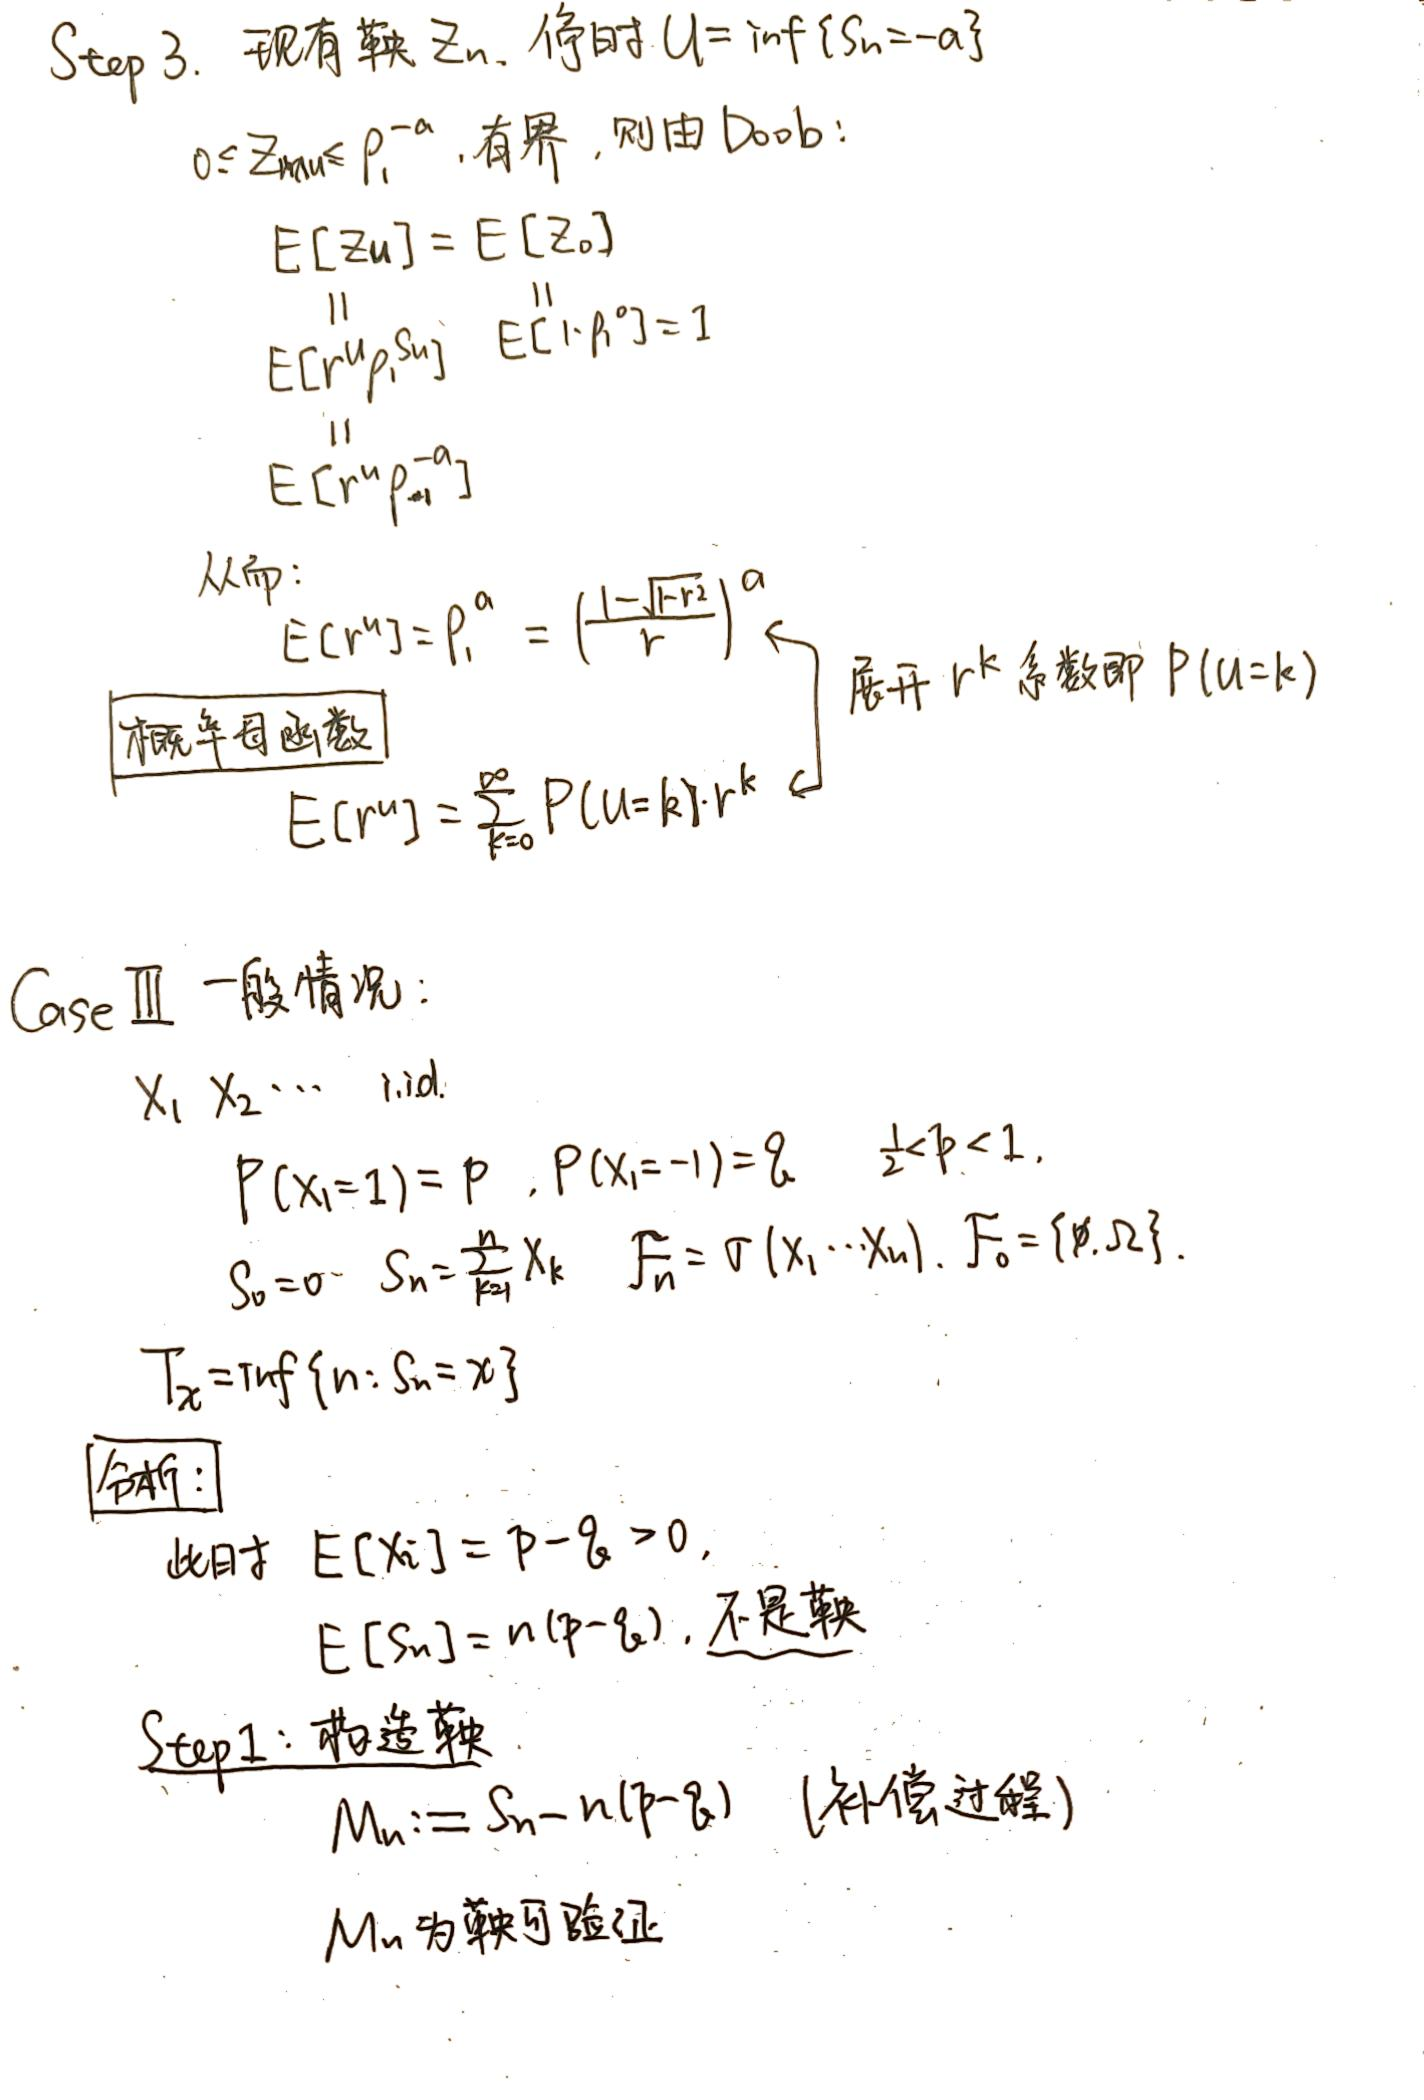
\includegraphics[width=0.92\textwidth]{3.jpg}
	\caption{步骤 3:边界条件与通解结构(示意)}\label{fig:rw-step3}
\end{figure}

\begin{figure}[h]
	\centering
	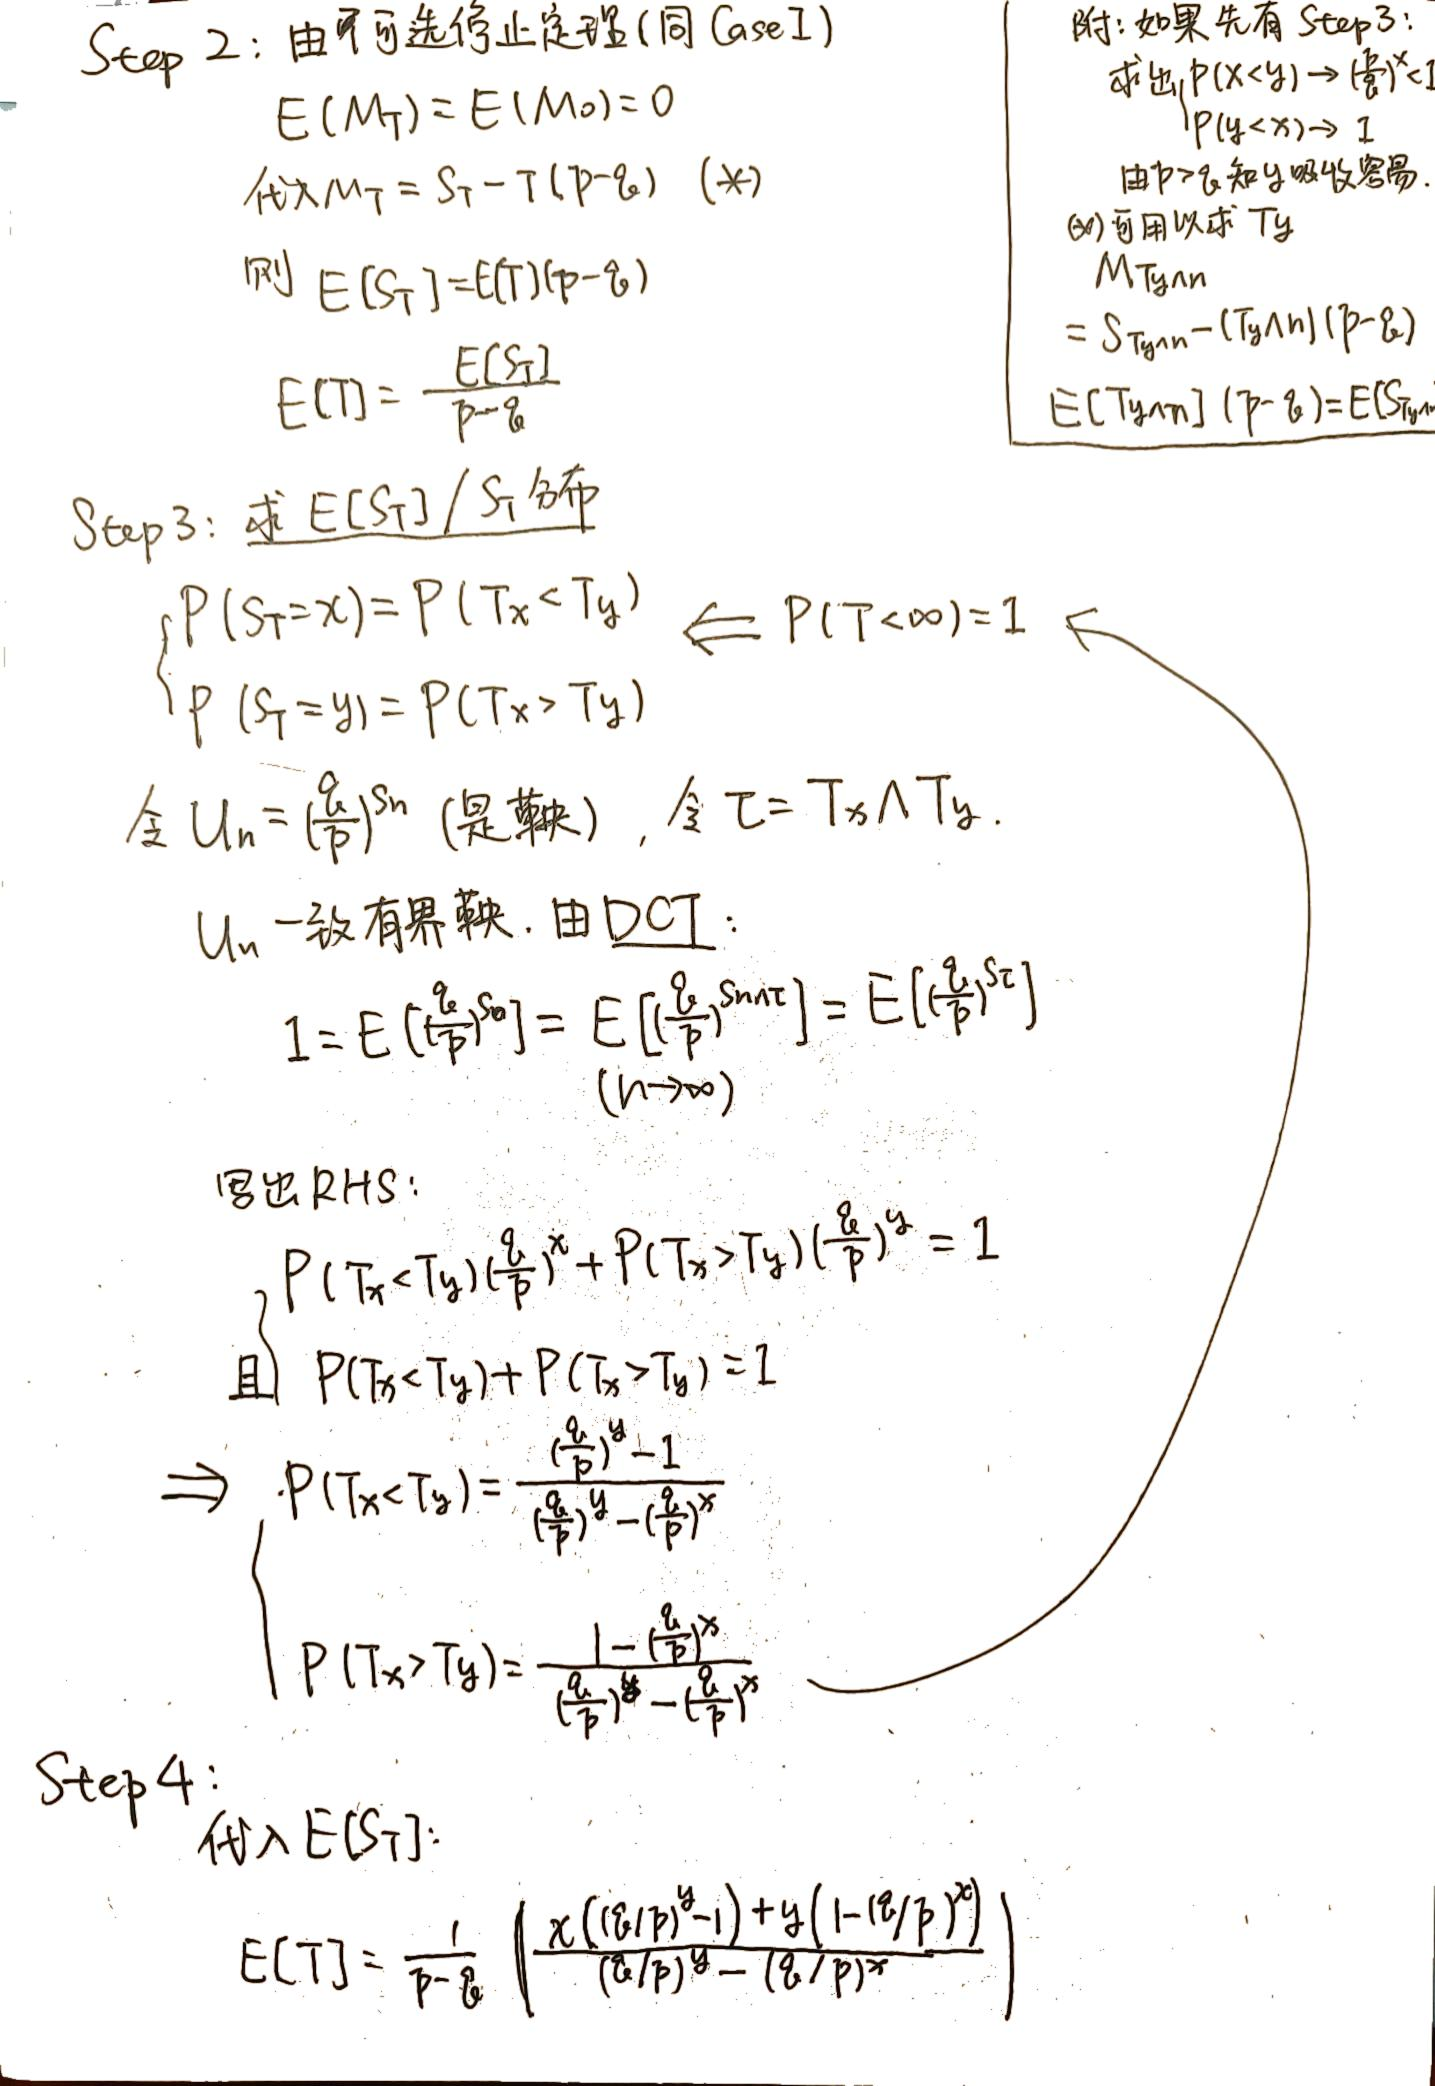
\includegraphics[width=0.92\textwidth]{4.jpg}
	\caption{步骤 4:常数确定与概率/期望解(示意)}\label{fig:rw-step4}
\end{figure}

\begin{figure}[h]
	\centering
	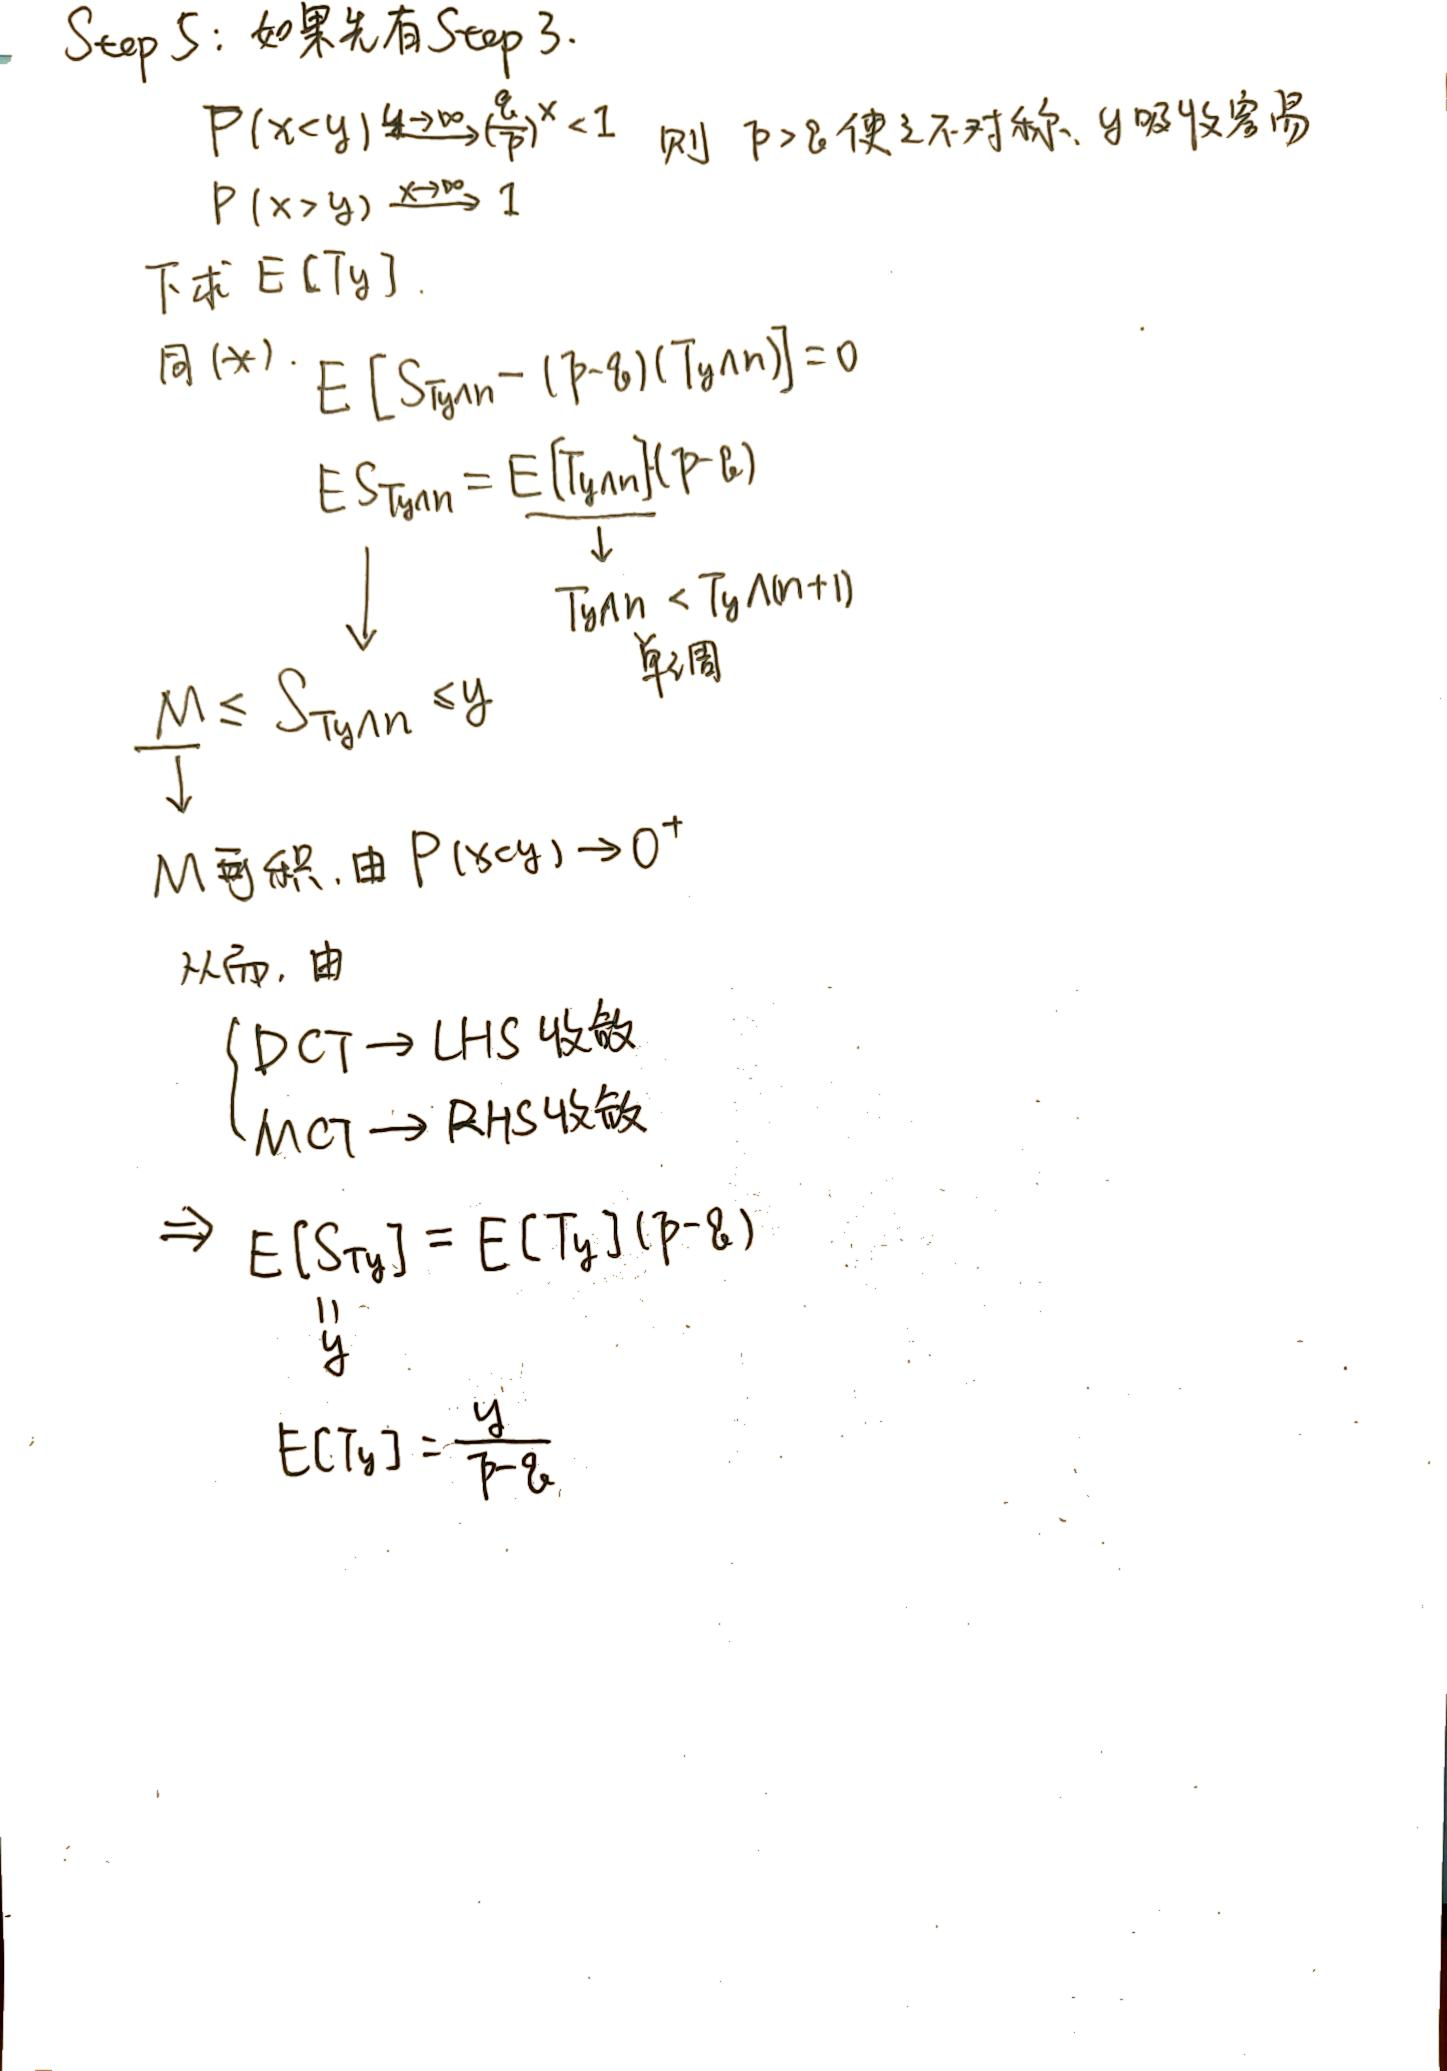
\includegraphics[width=0.92\textwidth]{5.jpg}
	\caption{步骤 5:结论与特殊情形讨论(示意)}\label{fig:rw-step5}
\end{figure}

\vspace{1em}
\noindent
如需将每一步转写为可检验的公式推导,我可以基于你的文字或草图内容补齐相应的差分/边值问题与闭式解,并将证明与说明整理为定理-推论-例题的结构。

\end{document}
